Genetsko programiranje podvrsta je genetskog algoritma. Najveća razlika između genetskog programiranja i genetskog algoritma je ta da je kod genetskog algoritma rješenje, odnosno jedinka, nepromjenjive duljine tijekom čitavog procesa evolucije.

U genetskom algoritmu, jedinka je predstavljena nizom informacija, primjerice nizom znamenki ili znakova, dok je kod genetskog programiranja jedinka predstavljena nekim slobodnijim oblikom, najčešće stablastom strukturom. Stablasta struktura pritom može predstavljati izvršivi program ili pak neki logički ili matematički izraz. Osim najčešće stablaste strukture, jedinka genetskog programiranja također može biti predstavljena i linearno, nizom informacija promjenjive duljine (primjerice, u slučaju da jedinka predstavlja program, može biti predstavljena nizom izvršivih instrukcija).

\section{Tijek algoritma}

Sam algoritam genetskog programiranja oponaša prirodnu evoluciju. Nakon stvaranja, skup jedinki koji čini populaciju algoritma, prolazi kroz proces evolucije pronalazeći rješenje danog problema. Tijek algoritma prikazan je na slici \ref{tijek}.

Algoritam započinje inicijalizacijom početne populacije rješenja, odnosno jedinki. Nakon stvaranje početne populacije, potrebno je evaluirati svaku zasebnu jedinku. Evaluacija se pritom odnosi na izračun dobrote (\textit{eng. fitness}) jedinke; svojstva koje govori o tome koliko je ona kvalitetno rješenje. Pomoću dobrote, jedinke su međusobno usporedive.

Inicijalizacijom populacije započinje prva generacija algoritma. Na početku svake generacije provjerava se da li je zadovoljen kriterij zaustavljanja algoritma. Ukoliko je, algoritam završava sa svojim izvođenjem, a u suprotnom, sljedeći korak algoritma je selekcija jedinki. 
Selekcijom se odabiru jedinke koje će preživjeti i sudjelovati u križanju u ulozi roditelja, te jedinka koja će biti zamijenjena njihovim potomkom.

Nakon dobivanja nove jedinke križanjem, ona se mutira s određenom vjerojatnosti mutacije te se izračunava njena nova dobrota.

Ova tri operatora; selekcija, mutacija i križanje, predstavljaju imitaciju evolucije u samom algoritmu. Isto kao u prirodi, u sljedeću generaciju ulaze samo najjače jedinke čiji se genetski materijal kombinira u nešto novo, pokušavajući naći kombinaciju materijala koja će donijeti poboljšanje.


\begin{figure}[H]
	\centering
	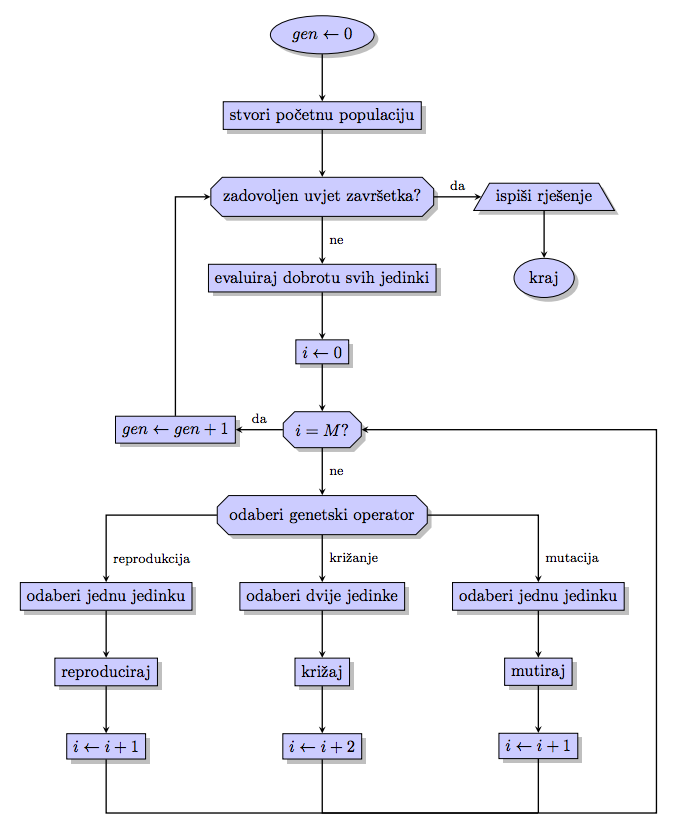
\includegraphics[scale=0.6]{./slike/blokDijagram.png}
	\caption{Tijek izvršavanja algoritma genetskog programiranja (slika preuzeta iz \cite{kokan})}
	\label{tijek}
\end{figure}

\section{Stablasta jedinka}
Najčešći oblik jedinke korišten u genetskom programiranju je stablo. Razlog zašto je tome tako je činjenica da se stablo može interpretirati na više različitih način. Stablo je pogodno za prikaz programskih jedinki, kao i prikaz jedinki koji predstavljaju neki matematički ili logički izraz.


\subsection{Stablo kao program}
Pomoću stabla lako je modelirati neki izvršivi program. Jedan od poznatijih problema rješavanih genetskim programiranjem je problem umjetnog mrava (\textit{eng. Artificial ant problem} \cite{koza}). U ovom slučaju, jedinka predstavlja ponašanje mrava unutar neke okoline. Cilj algoritma je evoluirati ponašanje koje će efikasno pronalaziti hranu unutar te okoline.

 Nezavršni znakovi unutar stabla pritom donose odluke o ponašanju, dok završni znakovi predstavljaju samo ponašanje pojedinog mrava. Na slici \ref{ant} prikazana je jedna takva jedinka. 

\begin{figure}
	\centering

\begin{tikzpicture}
[sibling distance=50mm, level distance=25mm,
every node/.style={fill=blue!20,rectangle, rounded corners,draw,drop shadow, minimum height=1.5cm}]


  \node {ifFoodAhead}
      child {node {moveForward}}
      child {node {Prog2}
        child {node {turnRight}}
        child {node {ifFoodAhead}
        	child{node {moveForward}}
        	child{node {turnLeft}}
        }
      };
\end{tikzpicture}

	\caption{Primjer jedinke programa umjetnog mrava}
	\label{ant}
\end{figure}


Nezavršni znakovi koji grade jednu ovakvu jedinku su:

\begin{enumerate}

  \item \textbf{If food ahead} - provjerava da li se nalazi hrana ispred mrava - ako da izvršava lijevu granu, ako ne, izvršava desnu granu.
  \item \textbf{Prog2} - slijedno izvršava lijevu, te zatim desnu granu.
  \item \textbf{Prog3} - slijedno izvršava (s lijeva na desno) svaku od 3 pridružene grane.

\end{enumerate}

Završni znakovi koji grade ovu jedinku su:
\begin{enumerate}

  \item \textbf{move forward} - pomiče mrava za jedno mjesto unaprijed.
  \item \textbf{turn right} - okreće mrava u desno.
  \item \textbf{turn left} - okreće mrava u lijevo.

\end{enumerate}

Ovakva stabla vrlo je jednostavno za interpretirati - kreće se od vršnog čvora, te se prema pravilima čvorova prolazi kroz stablo i izvršavaju dane instrukcije. Pseudokod koji opisuje stablo prikazano na slici \ref{ant} dan je ispod (\ref{pseudokod}).

\begin{algorithm}
\eIf {food ahead} {
	move forward;
} {
	turn right;\\
	\eIf {food ahead} {
		move forward;
	} {
		turn left;
	}
}

	\caption{Pseudokod jedinke prikazane na slici \ref{ant}}
	\label{pseudokod}
	\centering
\end{algorithm}

\subsection{Stablo kao logički izraz}

Osim programa, stablo može reprezentirati i neki logički izraz. Pri tome, nezavršni čvorovi predstavljaju logičke funkcije, dok završni čvorovi predstavljaju varijable. Logička funkcija predstavljena takvim stablom jednostavno se može izlučiti \textit{in-order} obilaskom stabla. Jedna ovakva jedinka dana je na slici \ref{logTree}. 
\\
\begin{figure}[H]
	\centering
	\begin{tikzpicture}
	[sibling distance=30mm, level distance=20mm,
	every node/.style={fill=blue!20,circle,draw,drop shadow, minimum height=1.5cm}]
	\node {\textbf{AND}}
    		child {node {A}}
    		child {node {\textbf{OR}}
        		child {node {B}}
        		child {node {C}}
      		};
	\end{tikzpicture}
	\caption{Stablo koje predstavlja logički izraz $A  \cdot (B + C)$}
	\label{logTree}
\end{figure}


\subsection{Stablo kao matematički izraz}

Jednako kao i logičke izraze, stablo može predstavljati neki matematički izraz. Kao i u prethodnom slučaju, matematički izraz se iz stabla može izlučiti \textit{in-order} obilaskom. Na slici \ref{matTree} prikazana je jedna takva jedinka.

\begin{figure}[H]
	\centering
	\begin{tikzpicture}
	[sibling distance=30mm, level distance=20mm,
	every node/.style={fill=blue!20,circle,draw,drop shadow, minimum height=1.5cm}]
	\node {\textbf{+}}
    		child {node {a}}
    		child {node {\textbf{$\cdot$}}
        		child {node {2}}
        		child {node {y}}
      		};
	\end{tikzpicture}
	\caption{Stablo koje predstavlja matematički izraz $a + 2 \cdot y$}
	\label{matTree}
\end{figure}

\section{Dobrota jedinke}

Dobrota (\textit{eng. fitness}) jedinke predstavlja njenu kvalitetu - označava koliko dobro ta jedinka rješava dani problem. Dobrota je najčešće predstavljena realnim brojem, te omogućuje mođusobnu usporedivost jedinki. Na osnovi iznosa dobrote pojedine jedinke provodi se selekcija unutar populacije.

Definiranje funkcije dobrote kojom se dobiva sam iznos dobrote jedan je od problema koji se pojavljuje prilikom postavljanja samog algoritma. Funkcija dobrote razlikuje se za svaki pojedini problem.

 Lako je uočljivo kako dobrota uvelike definira smjer napretka algoritma, te je stoga pitanje pronalaska adekvatne funkcije dobrote vrlo važno za kvalitetu samog algoritma. 

\section{Operatori selekcije}
Selekcija u genetskom programiranju osigurava prijenos kvalitetnog genetskog materijala u buduće generacije birajući jedinke koje će sudjelovati u reprodukciji  \cite{nenr}. Operatori selekcije se prema metodi odabira jedinki dijele na:

\begin{itemize}
\item proporcionalne selekcije - odabiru jedinke s vjerojatnošću koja je proporcionalna njihovoj dobroti
\item rangirajuće selekcije - odabiru jedinke s vjerojatnošću koja ovisi o rangu  dobrote jedinke (u usporedbi s dobrotama ostalih jedinki)
\end{itemize}

Ovisno o načinu prenošenja genetskog materijala boljih jedinki u iduću iteraciju načini selekcije se dijele na:

\begin{itemize}
	\item generacijske selekcije - selekcija direktno bira bolje jedinke koje sudjeluju u križanju
	\item eliminacijske selekcije - selekcija bira lošije jedinke za eliminaciju; bolje jedinke 				u ovom slučaju preživljavaju selekciju
\end{itemize}

\subsection{Generacijska selekcija}

Generacijska selekcija direktno odabire dvije jedinke koje će sudjelovati u reprodukciji, kopirajući one bolje jedinke u novu populaciju - nazvanu međupopulacijom. Broj jedinki u međupopulaciji manji je nego onaj u originalnog populaciji. Budući da sve jedinke populacije neće preživjeti selekciju, u međupopulaciju se najčešće stavljaju duplikati preživjelih jedinki. Iz ovoga se vidi očiti problem koji nastaje ovakvom selekcijom - smanjuje se raznovrsnost genetskog materijala koji će sudjelovati u reprodukciji. Posljedično, nedostatak genetske raznovrsnosti doprinosi usporavanju procesa evolucije.

Iz opisanog je vidljivo kako generacijska selekcija stvara čvrstu granicu između generacija - svaka jedinka postoji točno jednu generaciju.


\subsection{Eliminacijska selekcija}

Za razliku od generacijske selekcije, kod koje postoji čvrsta granica između generacija, u eliminacijskoj selekciji dobre jedinke preživljavaju više generacija. Eliminacijska selekcija nadomješta \textit{M} jedinki novim jedinkama koje su nastale reprodukcijom onih boljih. Pri tome, parametar \textit{M} se naziva mortalitetom.

Eliminacijska selekcija svojim djelovanjem ne stvara duplikate jedinki čime se otklanja osnovni problem generacijske selekcije.

\section{Operatori križanja}

Operatori križanja obavljaju rekombinaciju genetskog materijala, stvarajući jednu novu jedinku koja nastaje kombinacijom neke druge dvije, roditeljske jedinke. U slučaju genetskog programiranja gdje je jedinka predstavljena u obliku stabla, križanje se svodi na spajanje dvaju podstabla roditelja u novo stablo djeteta (slika \ref{crx}). Zasebni operatori križanja detaljno će biti opisani u idućem poglavlju.

\begin{figure}[H]
 	\centering


	\begin{tikzpicture}
	[sibling distance=25mm, level distance=15mm,
	every node/.style={fill=blue!20,circle,draw,drop shadow, minimum height=1cm}]
	\node {\textbf{+}}
    		child {node {a}}
    		child {node {\textbf{$\cdot$}}
        		child {node {2}}
        		child {node {y}}
      		};
	};

\begin{scope}[xshift=7cm]
	\node {\textbf{+}}
    		child {node {a}
        		child {node {2}}
        		child {node {y}}
      		}
    		child {node {\textbf{$sin$}}
			child {node {x}}};
	};
\end{scope}

\begin{scope}[xshift=11.5cm]

	\node  {\textbf{+}}
    		child {node {a}}
    		child {node {\textbf{$sin$}}
        		child {node {x}}
      		};
	};

\end{scope}
	\end{tikzpicture}


	\caption{Primjer jednostavnog križanja stabala}
	\label{crx}
\end{figure}


\section{Operatori mutacije}

Mutacija je operator koji djeluje direktno na pojedinu jedinku. Kao i u prirodi, mijenja jedan dio jedinke. Jedinka mutira s određenom vjerojatnošću, koji je uobičajeno broj reda veličine 0.1. Na slici \ref{mutSimple} prikazana je jednostavna mutacija koja nasumično mijenja jedan čvor stabla. 

Uobičajene metode mutacije uključuju:

\begin{itemize}
	\item zamjena nasumično odabranog podstabla novim, također nasumično generiranim stablom
	\item zamjena nasumično odabranog čvora njegovim komplementom
	\item zamjena slučajno odabranog čvora čvorom istog tipa
	\item zamjena slučajno odabranog podstabla završnim čvorom
\end{itemize}
\begin{figure}[H]
 	\centering


\begin{tikzpicture}
	[sibling distance=25mm, level distance=15mm,
	every node/.style={fill=blue!20,circle,draw,drop shadow, minimum height=1cm}]

\begin{scope}[xshift=0cm]
	\node   {\textbf{+}}
    		child {node {$cos$}
    			child {node {-}
    				child {node {x}}
    				child {node {y}}
    			}
    		}
    		child {node {\textbf{$/$}}
			child {node  {x}}
			child {node  {y}}	
		};
	};
\end{scope}

\begin{scope}[xshift=7cm]
	\node   {\textbf{+}}
    		child {node [fill=red!20] {$sin$}
    			child {node {-}
    				child {node {x}}
    				child {node {y}}
    			}
    		}
    		child {node {\textbf{$/$}}
			child {node  {x}}
			child {node  {y}}	
		};
	};
\end{scope}

\end{tikzpicture}


	\caption{Primjer jednostavne mutacije. Desno: jedinka prije mutacije, lijevo: jedinka nakon mutacije}
	\label{mutSimple}
\end{figure}

Mutacija je vrlo korisna u slučaju kada jedinka zapne u nekom od lokalnih minimuma. Naime, mutacija može značajno promijeniti jedinku, te ju tako dosta udaljiti od trenutnog prostora pretraživanja. 
